\documentclass[11pt,a4paper]{article}

% --- Packages ---
\usepackage[margin=1in]{geometry}
\usepackage{amsmath,amssymb,amsthm}
\usepackage{mathtools}
\usepackage{bm}
\usepackage{graphicx}
\usepackage{hyperref}
\usepackage{cleveref}
\usepackage{booktabs}
\usepackage{enumitem}
\usepackage{xcolor}
\usepackage[numbers]{natbib}
\usepackage{algorithm}
\usepackage{algpseudocode}

% --- Theorem Environments ---
\newtheorem{proposition}{Proposition}
\newtheorem{definition}{Definition}
\newtheorem{remark}{Remark}
\newtheorem{assumption}{Assumption}

% --- Custom Commands ---
\newcommand{\hv}{\mathbf{h}}
\newcommand{\bx}{\mathbf{x}}
\newcommand{\bn}{\mathbf{n}}
\newcommand{\br}{\mathbf{r}}
\newcommand{\bs}{\mathbf{s}}
\newcommand{\bW}{\mathbf{W}}
\newcommand{\cN}{\mathcal{N}}
\newcommand{\cI}{\mathcal{I}}
\newcommand{\cE}{\mathcal{E}}
\newcommand{\cH}{\mathcal{H}}
\newcommand{\cC}{\mathcal{C}}
\newcommand{\cV}{\mathcal{V}}
\newcommand{\cP}{\mathcal{P}}
\newcommand{\Rad}{\text{Radicalization}}

% -------------------------------------------------------
\title{%
  \textbf{SimCity: A Unified Neural-Epidemiological Architecture} \\
  \large for Modelling Viral Information Dynamics on Multiplex Internet Graphs
}
\author{[Author Names]}
\date{}
% -------------------------------------------------------

\begin{document}
\maketitle

\begin{abstract}
The dynamics of internet virality exhibit both macroscopic epidemiological
patterns and microscopic, graph-structural volatility. Current literature largely
isolates these domains: macroscopic models (e.g., SEIR) fail to capture the
transient topology of social networks, while microscopic graph models
(e.g., Temporal Graph Networks) lack population-level infection dynamics. In
this paper, we present \textbf{SimCity}, a unified neural-epidemiological
architecture that bridges this gap. We introduce a Stochastic SEIR-Z-D
compartmental model grounded by a Degree-Correlated Heterogeneous Mean-Field
(HMF) approximation, which maps continuous-time Temporal Graph Network (TGN)
embeddings directly into epidemiological transition rates. We couple this with a
Neural Multivariate Hawkes Process for cross-platform narrative transfer and a
Filippov-compliant smooth Deffuant model for agent behavioural evolution.
Empirically, we make three contributions: (1) we show that raw engagement-count
regression --- the de-facto virality metric --- is intrinsically noise-dominated
under near-critical cascade dynamics (even an oracle handed the true excitation
state attains negative residual skill), arguing for timing- and transfer-based
evaluation; (2) on a controlled multiplex benchmark with ground-truth
cross-platform excitation, our narrative-conditioned intensity model detects
\emph{which} narratives will transfer across platforms (AUC $0.653 \pm 0.005$
over three seeds, $p < 1.1\times10^{-4}$, robust to popularity and reach
confounds) --- a task on which any static Hawkes process is random by
construction; and (3) this transfer result replicates on a balanced live Hacker
News + GDELT corpus (AUC 0.632, $p = 1.2\times10^{-3}$), above a popularity
baseline, using a released accumulating collector.
\end{abstract}

% =============================================================
\section{Related Work}
\label{sec:related}
% =============================================================

\paragraph{Temporal graph representation learning.}
Continuous-time dynamic graph models embed evolving interaction streams:
JODIE~\citep{kumar2019predicting} learns coupled user/item trajectories,
DyRep~\citep{trivedi2019dyrep} drives embeddings with a two-time-scale point
process, TGAT~\citep{xu2020tgat} introduces functional time encoding for
temporal attention, and TGN~\citep{rossi2020temporal} unifies these with a
memory module, which we adopt as our structural backbone. These models are
trained for link-level prediction; they contain no population-level infection
dynamics and no mechanism for platform-to-platform transfer, which is precisely
the gap SimCity's HMF bridge (\cref{sec:hmf}) and cross-platform Hawkes head
(\cref{sec:hawkes}) address.

\paragraph{Hawkes processes and neural temporal point processes.}
Self- and mutually-exciting processes~\citep{hawkes1971spectra} underpin much of
social-media modelling. Neural parameterisations replace fixed kernels with
learned dynamics: RMTPP~\citep{du2016rmtpp}, the Neural Hawkes
Process~\citep{mei2017neural}, and the Transformer Hawkes
Process~\citep{zuo2020transformer}. Closer to our setting,
NETRATE~\citep{gomez2011netrate} infers diffusion networks from cascades,
COEVOLVE~\citep{farajtabar2017coevolve} couples diffusion with network growth,
and prior work separates endogenous from exogenous
influence~\citep{myers2012external} --- our GDELT-driven $\mu_i(t)$ follows
this exogenous/endogenous decomposition.
Our contribution is orthogonal to kernel expressiveness: we condition the
\emph{cross-platform excitation matrix itself} on evolving graph and narrative
state, which is what enables per-narrative transfer ranking
(\cref{sec:results}) --- a static or globally-parameterised Hawkes model is
random at that task by construction.

\paragraph{Cascade and popularity prediction.}
Feature-based and deep models predict cascade size: cascade growth was framed
as a prediction problem in~\citep{cheng2014cascades},
SEISMIC~\citep{zhao2015seismic} and Hawkes intensity
processes~\citep{rizoiu2017hip,kobayashi2016tideh} model retweet dynamics,
reinforced Poisson processes model item popularity~\citep{shen2014rpp}, and
DeepCas/DeepHawkes~\citep{li2017deepcas,cao2017deephawkes} learn end-to-end
representations; community structure also signals virality~\citep{weng2013virality}.
Our negative result (\cref{sec:results}) complements this line: under
near-critical branching, next-window \emph{counts} are noise-dominated even for
an oracle, motivating timing- and transfer-based evaluation instead of raw
magnitude regression.

\paragraph{Epidemic models on networks.}
Degree-based mean-field theory characterises epidemic thresholds on
heterogeneous graphs~\citep{pastor2001epidemic,boguna2002correlated,pastor2015epidemic}.
We import the degree-correlated HMF closure into a learned setting, using TGN
embeddings to supply node-level infectivities that are aggregated into
macroscopic SEIR-Z-D rates --- to our knowledge the first bridge from
continuous-time graph memory states to compartmental transition rates.

\paragraph{Cross-platform information flow.}
Empirical work documents inter-platform influence: the ``web
centipede''~\citep{zannettou2017webcentipede} traces news trajectories across
communities, coordinated cross-platform disinformation campaigns have been
analysed in~\citep{wilson2020crossplatform}, platform migrations reshape community
behaviour~\citep{horta2021migrations}, and false news spreads with distinctive
dynamics~\citep{vosoughi2018spread}. These studies are measurement-focused;
SimCity provides the corresponding \emph{predictive} instrument --- a causal,
per-narrative transfer score evaluated prospectively on live Hacker News +
GDELT data.

\paragraph{Opinion dynamics.}
Bounded-confidence models~\citep{deffuant2000mixing,hegselmann2002opinion} and
their statistical-physics treatments~\citep{castellano2009statistical} evolve
continuous opinions under confidence thresholds. We contribute a
Filippov-compliant smooth relaxation (\cref{sec:deffuant}) whose radicalization
state feeds back into representation learning, coupling behavioural and
structural dynamics.

% =============================================================
\section{Information Propagation: Stochastic SEIR-Z-D Model}
\label{sec:seir}
% =============================================================

To rigorously capture the volatile, non-deterministic nature of viral information
spread, we formulate a continuous-time Stochastic Master Equation (SME). We
introduce a \textbf{Zombie} ($Z$) state to model algorithmic resurfacing, and an
\textbf{Archived/Dead} ($D$) absorbing state to ensure population conservation
and a well-defined long-run limit.

\subsection{State Definitions and Population Conservation}

Let the network state at time $t$ be defined by the discrete random variable
vector
\[
  \bn(t) = (n_S,\, n_E,\, n_I,\, n_R,\, n_Z,\, n_D).
\]
The six compartments are:
\begin{itemize}[noitemsep]
  \item $S$ (Susceptible): users who have not yet encountered the content.
  \item $E$ (Exposed): users who have seen the content but not yet shared it.
  \item $I$ (Infected): users actively sharing and propagating the content.
  \item $R$ (Recovered): users who have lost interest (decayed engagement).
  \item $Z$ (Zombie): content resurfaced from $R$ via algorithmic recommendation
        or external shock.
  \item $D$ (Archived/Dead): content in a final absorbing state; no further
        transitions are possible.
\end{itemize}
We explicitly enforce a \emph{constant} total population:
\begin{equation}
  N \;=\; n_S(t) + n_E(t) + n_I(t) + n_R(t) + n_Z(t) + n_D(t)
  \quad \forall\, t.
  \label{eq:conservation}
\end{equation}

\begin{remark}
On the internet $N$ is not strictly constant (new accounts, lurkers becoming
active). We treat $N$ as fixed throughout a single cascade window, a standard
simplification in compartmental internet models. Extensions to open populations
are left as future work.
\end{remark}

\subsection{Transition Rates and Jump Vectors}
\label{sec:transitions}

The system evolves via five discrete transitions. Each is characterised by a
transition rate $W_k(\bn)$ and a state jump vector $\br_k \in \mathbb{Z}^6$.

\begin{enumerate}[label=\textbf{T\arabic*.}, leftmargin=*, noitemsep]

  \item \textbf{Exposure} ($S \to E$): \quad
        $\br_1 = (-1,\;{+1},\;0,\;0,\;0,\;0)$
        \begin{equation}
          W_1(\bn) \;=\; \beta(t)\cdot
          \frac{n_S\bigl(n_I + \theta\, n_Z\bigr)}{N},
          \label{eq:w1}
        \end{equation}
        where $\theta \ge 0$ scales the algorithmic boost of resurfaced zombie
        content.

  \item \textbf{Activation} ($E \to I$): \quad
        $\br_2 = (0,\;-1,\;{+1},\;0,\;0,\;0)$
        \begin{equation}
          W_2(\bn) \;=\; \sigma\, n_E.
          \label{eq:w2}
        \end{equation}

  \item \textbf{Decay} ($I \to R$): \quad
        $\br_3 = (0,\;0,\;-1,\;{+1},\;0,\;0)$
        \begin{equation}
          W_3(\bn) \;=\; \gamma_I\, n_I.
          \label{eq:w3}
        \end{equation}

  \item \textbf{Resurgence} ($R \to Z$): \quad
        $\br_4 = (0,\;0,\;0,\;-1,\;{+1},\;0)$
        \begin{equation}
          W_4(\bn) \;=\; \zeta(t)\, n_R,
          \label{eq:w4}
        \end{equation}
        where $\zeta(t)$ is driven by cross-platform narrative shocks;
        see \cref{sec:hawkes} for the formal link.

  \item \textbf{Archival} ($Z \to D$): \quad
        $\br_5 = (0,\;0,\;0,\;0,\;-1,\;{+1})$
        \begin{equation}
          W_5(\bn) \;=\; \delta_D\, n_Z.
          \label{eq:w5}
        \end{equation}
        $D$ is absorbing: no outgoing transitions exist, closing the
        $Z \to R$ infinite-loop present in standard SEIR-Z formulations.

\end{enumerate}

\begin{remark}
The decay parameter in \textbf{T3} is denoted $\gamma_I$ to avoid confusion with
the Hawkes decay parameter $\hat{\gamma}_{ij}$ introduced in \cref{sec:hawkes}.
\end{remark}

\subsection{The Master Equation}

The time evolution of the joint probability distribution $P(\bn, t)$ is governed
by:
\begin{equation}
  \frac{dP(\bn, t)}{dt}
  \;=\;
  \sum_{k=1}^{5}
  \Bigl[
    W_k(\bn - \br_k)\,P(\bn - \br_k,\, t)
    \;-\;
    W_k(\bn)\,P(\bn,\, t)
  \Bigr].
  \label{eq:master}
\end{equation}
This formulation fully specifies the Markov process: each term represents
probability \emph{flowing into} state $\bn$ from $\bn - \br_k$ minus probability
\emph{leaving} $\bn$ via transition $k$. Taking expectations over $P(\bn, t)$
recovers the macroscopic ODEs, while the second moment yields virality variance.

% =============================================================
\section{Micro-Dynamics: Temporal Graph Network Integration}
\label{sec:tgn}
% =============================================================

The macroscopic rates $\beta(t)$ and $\zeta(t)$ are \emph{not} static parameters;
they are derived dynamically from the evolving micro-structure of the social
graph via a Temporal Graph Network (TGN) augmented with a
\textbf{Virality Prediction Head}.

\subsection{Core TGN (Rossi et al., 2020)}

For a node $v$ involved in an interaction with node $u$ at time $t$:
\begin{align}
  \text{Message:} \quad
    \bs_v(t) &= \mathrm{GRU}\!\left(\bs_v(t^-),\;
               \bar{m}_v(t)\right), \label{eq:tgn-mem}\\
  \text{where} \quad
    m_v(t) &= \mathrm{Msg}\!\left(\bs_v(t^-),\;\bs_u(t^-),\;
              \Delta t,\; e_{vu}(t)\right), \notag\\
  \text{Embedding:} \quad
    \hv_v(t) &= \mathrm{attn}\!\left(\bs_v(t),\;
               \{\bs_u(t)\}_{u\in\cN(v)}\right). \label{eq:tgn-emb}
\end{align}

\subsection{Contextual Content Embedding}
\label{sec:content-emb}

Content $c$ is not a static entity; its contextual embedding evolves as users
interact with it. To prevent self-referential circularity, attention weights are
computed strictly from \emph{pre-update} historical embeddings $\hv(t^-)$:
\begin{equation}
  a_{u,c} \;=\;
  \frac{
    \exp\!\bigl(\hv_u(t^-)^\top \bW_a\, \hv_c(t^-)\bigr)
  }{
    \displaystyle\sum_{j\in\cN_c(t)}
    \exp\!\bigl(\hv_j(t^-)^\top \bW_a\, \hv_c(t^-)\bigr)
  },
  \label{eq:attn}
\end{equation}
\begin{equation}
  \hv_c(t) \;=\; \mathrm{GRU}\!\!\left(
    \hv_c(t^-),\;
    \sum_{u\in\cN_c(t)} a_{u,c}\;\hv_u(t^-)
  \right).
  \label{eq:content-emb}
\end{equation}
At $t=0$, content is initialised as
\begin{equation}
  \hv_c(0) \;=\; \bW_{\mathrm{proj}}\cdot\mathrm{LLM\_Encode}(\text{text}),
  \label{eq:content-init}
\end{equation}
where the LLM encoder is \emph{frozen} to prevent catastrophic forgetting, and
$\bW_{\mathrm{proj}}$ is a learned linear projection mapping the LLM output
dimension to the TGN hidden dimension $d$.

\subsection{Virality Prediction Head}
\label{sec:virality-head}

Node and content embeddings are mapped to predictive epidemiological and Hawkes
parameters via localised MLPs with Softplus output activations (enforcing
positivity):
\begin{align}
  \hat{\beta}_{v,c}(t) &= \mathrm{Softplus}\!\left(
    \mathrm{MLP}_\beta\!\left(\hv_v(t) \,\|\, \hv_c(t)\right)
  \right), \label{eq:beta-hat}\\
  \hat{\alpha}_{ij}(t) &= \mathrm{Softplus}\!\left(
    \mathrm{MLP}_\alpha\!\left(
      \hv_{\cP_i}(t) \,\|\, \hv_{\cP_j}(t) \,\|\, \hv_c(t)
    \right)
  \right), \label{eq:alpha-hat}\\
  \hat{\gamma}_{ij}(t) &= \mathrm{Softplus}\!\left(
    \mathrm{MLP}_\gamma\!\left(
      \hv_{\cP_i}(t) \,\|\, \hv_{\cP_j}(t) \,\|\, \hv_c(t)
    \right)
  \right), \label{eq:gamma-hat}
\end{align}
where $\hv_{\cP_i}(t)$ is the platform-level embedding defined in
\cref{sec:platform-emb}, $\hat{\beta}_{v,c}(t)$ feeds the HMF bridge
(\cref{sec:hmf}), and $\hat{\alpha}_{ij}(t)$, $\hat{\gamma}_{ij}(t)$ feed the
Neural Hawkes process (\cref{sec:hawkes}).

\subsection{Platform-Level Embedding}
\label{sec:platform-emb}

To aggregate node-level embeddings into platform-level representations for the
Hawkes infectivity MLPs, we use \textbf{Influence-Weighted Attention Pooling}.
Simple mean pooling would wash out super-spreader signals in heavy-tailed graphs;
instead, we weight by the dynamic influence score $I(v,t)$
(defined in \cref{sec:influence}):
\begin{equation}
  \hv_{\cP_i}(t) \;=\;
  \sum_{v\in V_{\cP_i}(t)}
  \alpha_v(t)\;\hv_v(t),
  \qquad
  \alpha_v(t) = \frac{
    \exp\!\bigl(\tau\cdot I(v,t)\bigr)
  }{
    \displaystyle\sum_{u\in V_{\cP_i}(t)}
    \exp\!\bigl(\tau\cdot I(u,t)\bigr)
  },
  \label{eq:platform-emb}
\end{equation}
where $\tau$ is a learnable temperature parameter.

\subsection{Joint Optimisation: Homoscedastic Multi-Task Loss}
\label{sec:loss}

All three objectives are formulated as regression/continuous tasks to satisfy
the Gaussian likelihood assumption underlying Kendall et al.'s homoscedastic
uncertainty weighting~\citep{kendall2018multi}:
\begin{equation}
  \mathcal{L}
  \;=\;
  \frac{1}{2\sigma_1^2}\mathcal{L}_{\mathrm{TGN}}
  + \frac{1}{2\sigma_2^2}\mathcal{L}_{\mathrm{Hawkes}}
  + \frac{1}{2\sigma_3^2}\mathcal{L}_{\mathrm{Virality}}
  + \log(\sigma_1\sigma_2\sigma_3),
  \label{eq:joint-loss}
\end{equation}
where $\sigma_1,\sigma_2,\sigma_3 > 0$ are learnable noise parameters.

\paragraph{(1) TGN Structural Loss --- InfoNCE.}
To learn embeddings that discriminate temporal edges from noise, we use a
temporal contrastive loss with degree-proportional negative sampling
$P_n(v)\propto d_v$ (uniform sampling produces trivially easy negatives in
heavy-tailed graphs):
\begin{equation}
  \mathcal{L}_{\mathrm{TGN}}
  = -\!\!\!\sum_{(u,v,t)\in\cE}
  \log
  \frac{
    \exp\!\bigl(\hv_u(t)^\top \hv_v(t)\bigr)
  }{
    \exp\!\bigl(\hv_u(t)^\top \hv_v(t)\bigr)
    +\displaystyle\sum_{v_{\neg}\sim P_n}
    \exp\!\bigl(\hv_u(t)^\top \hv_{v_{\neg}}(t)\bigr)
  }.
  \label{eq:info-nce}
\end{equation}
We draw $M=20$ negatives per positive edge, following Rossi et al.~(2020) as a
baseline; a systematic ablation over $M\in[10,200]$ is left as future work.

\paragraph{(2) Hawkes Negative Log-Likelihood.}
\begin{equation}
  \mathcal{L}_{\mathrm{Hawkes}}
  = -\sum_{i=1}^{|\cP|}
  \left[
    \sum_{t_k^{(i)}} \log\lambda_i\!\left(t_k^{(i)}\right)
    - \int_0^T \lambda_i(t)\,dt
  \right].
  \label{eq:hawkes-nll}
\end{equation}
The compensator integral is tractable via the piecewise-recursive update
described in \cref{sec:tractability}.

\paragraph{(3) Virality Regression Loss.}
\begin{equation}
  \mathcal{L}_{\mathrm{Virality}}
  = \frac{1}{|\cC|}
  \sum_{c\in\cC}
  \Bigl(\log E_c - \log\hat{E}_c\Bigr)^2,
  \label{eq:virality-loss}
\end{equation}
where $E_c$ is the true cumulative engagement count and $\hat{E}_c$ is the
model's prediction.

% =============================================================
\section{The Micro-Macro Bridge: Degree-Correlated HMF}
\label{sec:hmf}
% =============================================================

The individual node-level predictions $\hat{\beta}_{v,c}(t)$ must be aggregated
into the macroscopic SEIR-Z-D exposure rate $\beta(t)$. A naive homogeneous
mean-field approximation assumes uncorrelated, exchangeable nodes --- a
catastrophic assumption for the highly assortative, heavy-tailed graphs
characteristic of social media.

\subsection{Full Degree-Correlated HMF Formulation}

Let $P(k'|k)$ be the conditional probability that a node of degree $k$ connects
to a node of degree $k'$. Stratifying infected nodes by degree and weighting by
the source degree $k'$ (the number of susceptible contacts an infected node of
degree $k'$ can reach):
\begin{equation}
  \beta(t)
  \;=\;
  \sum_{k}\sum_{k'}
  P(k'|k)\cdot k'\cdot
  \mathbb{E}_{v\in\cI_{k'}(t)}\!\left[\hat{\beta}_{v,c}(t)\right].
  \label{eq:hmf}
\end{equation}

\begin{assumption}[Stationarity of Mixing Structure]
To avoid the $\mathcal{O}(V^2)$ cost of recomputing $P(k'|k)$ at every event,
we estimate it as a static approximation over the full observation window. This
is justified because while individual node degrees $k_v(t)$ are highly dynamic,
the macroscopic assortative mixing structure of a given platform remains
approximately stationary over the timescale of a single cascade.
\end{assumption}

\subsection{Effective Temporal Degree}
\label{sec:temporal-degree}

Because normalised TGN attention weights sum to 1 by construction (softmax),
they cannot serve as a proxy for graph volume. Instead, we define the effective
temporal degree $k_v(t)$ directly from the event stream within the TGN's
explicit memory horizon $\Delta T_{\mathrm{mem}}$:
\begin{equation}
  k_v(t)
  \;=\;
  \left|\bigl\{
    u\in\cV
    \;\big|\;
    \exists\;\text{interaction }(v,u,\tau):\;
    t - \Delta T_{\mathrm{mem}} \le \tau \le t
  \bigr\}\right|.
  \label{eq:temporal-degree}
\end{equation}
This guarantees that hubs yield large $k_v(t)$ and lurkers yield
$k_v(t)\approx 0$, restoring physical validity to \cref{eq:hmf}.

% =============================================================
\section{Cross-Platform Transfer: Neural Multivariate Hawkes Process}
\label{sec:hawkes}
% =============================================================

Internet narratives migrate across platforms: a burst on Reddit triggers a
cascade on Twitter/X, which bleeds into mainstream news (GDELT). We model this
mutually exciting cross-platform transfer with a \textbf{Neural Multivariate
Hawkes Process}.

\subsection{Conditional Intensity Function}

Let $N_i(t)$ be the counting process of narrative events on platform $i
\in\{1,\ldots,|\cP|\}$. The conditional intensity given history $\cH_t$ is:
\begin{equation}
  \lambda_i(t)
  \;=\;
  \mu_i(t)
  + \sum_{j=1}^{|\cP|}
    \sum_{t_k^{(j)} < t}
    \hat{\alpha}_{ij}(t_k)\cdot
    \exp\!\Bigl(-\hat{\gamma}_{ij}(t_k)\bigl(t - t_k^{(j)}\bigr)\Bigr),
  \label{eq:hawkes-intensity}
\end{equation}
where:
\begin{itemize}[noitemsep]
  \item $\mu_i(t)$ is the exogenous background rate on platform $i$
        (see \cref{sec:gdelt} for its empirical definition);
  \item $\hat{\alpha}_{ij}(t_k)\ge 0$ is the dynamic infectivity of platform $j$
        on platform $i$ at event time $t_k$, output by $\mathrm{MLP}_\alpha$
        (\cref{eq:alpha-hat});
  \item $\hat{\gamma}_{ij}(t_k) > 0$ is the dynamic exponential decay, output
        by $\mathrm{MLP}_\gamma$ (\cref{eq:gamma-hat}).
\end{itemize}
When $j=i$, $\hat{\alpha}_{ii}$ captures \emph{intra-platform} self-excitation
(e.g., Reddit posts triggering more Reddit posts); $j\neq i$ captures
\emph{cross-platform} narrative transfer.

\begin{proposition}[Cascade Threshold]
Define the branching matrix $\bm{\Gamma}$ with entries
$\Gamma_{ij} = \hat{\alpha}_{ij}/\hat{\gamma}_{ij}$. A narrative exhibits
subcritical (fading) behaviour if the spectral radius $\rho(\bm{\Gamma}) < 1$.
If $\rho(\bm{\Gamma}) \ge 1$, the narrative goes globally viral.
\end{proposition}

\begin{proof}[Proof sketch]
For fixed parameters, $\Gamma_{ij} = \int_0^\infty
\hat{\alpha}_{ij} e^{-\hat{\gamma}_{ij} s}\, ds$ is the expected number of
platform-$i$ offspring of a platform-$j$ event, so $\bm{\Gamma}$ is the mean
offspring matrix of the associated multitype branching process; extinction
(stationarity of the linear Hawkes process) holds iff
$\rho(\bm{\Gamma}) < 1$~\citep{hawkes1971spectra,bremaud1996stability}. In our
model $\hat\alpha, \hat\gamma$ are piecewise-constant between events
(\cref{sec:tractability}), so the criterion applies locally per inter-event
interval; $\rho(\bm{\Gamma}(t))$ then acts as an instantaneous criticality
index rather than a global stationarity guarantee.
\end{proof}

\subsection{Linking $\zeta(t)$ to the Hawkes Process}

The resurgence rate $\zeta(t)$ in the SME (\cref{eq:w4}) is formally defined as
a function of the aggregate cross-platform Hawkes intensity on the content's
originating platform $i^*$:
\begin{equation}
  \zeta(t) \;=\; f\!\left(\lambda_{i^*}(t)\right)
  \;=\; \phi\cdot\max\!\left(0,\;\lambda_{i^*}(t) - \bar{\lambda}_{i^*}\right),
  \label{eq:zeta}
\end{equation}
where $\bar{\lambda}_{i^*}$ is the rolling baseline intensity and $\phi > 0$
is a scaling hyperparameter. Surges above baseline directly elevate the
probability of zombie resurgence.

\subsection{Piecewise-Recursive Tractability of the Compensator}
\label{sec:tractability}

Standard Hawkes processes with static $\alpha_{ij},\gamma_{ij}$ admit a single
closed-form compensator. In our model, $\hat{\alpha}_{ij}(t_k)$ and
$\hat{\gamma}_{ij}(t_k)$ are TGN outputs that update \emph{discretely} at each
event, remaining piecewise-constant between events. The exponential kernel then
permits a recursive analytical update: between consecutive events $t_k$ and
$t_{k+1}$, the integral contribution
\[
  \int_{t_k}^{t_{k+1}} \lambda_i(t)\,dt
\]
is closed-form given the fixed parameters at $t_k$, reducing the full
compensator to a tractable sum over event intervals.

% =============================================================
\section{Agent Behavioural Policy: Smooth Deffuant Model}
\label{sec:deffuant}
% =============================================================

For simulating node-level opinion evolution, we adapt the continuous-opinion
Deffuant model to (i) operate in continuous time and (ii) incorporate
platform-specific confidence bounds that shrink with user radicalization.

\subsection{Filippov-Compliant Smooth Formulation}

The standard Deffuant model uses a hard indicator function
$\mathbf{1}_{|x_v - x_c|\le\epsilon_p}$, which destroys Lipschitz continuity
and violates the Picard--Lindelöf existence and uniqueness theorem. We replace it
with a smooth logistic approximation:
\begin{equation}
  \dot{x}_v(t)
  \;=\;
  \eta\cdot\bigl(x_c - x_v(t)\bigr)\cdot
  \sigma\!\Bigl(\rho\cdot\bigl(\epsilon_p(v) - |x_v(t) - x_c|\bigr)\Bigr),
  \label{eq:deffuant}
\end{equation}
where $\sigma(z) = (1+e^{-z})^{-1}$, $\eta$ is the opinion convergence rate,
and the steepness hyperparameter is bound as
\begin{equation}
  \rho \;=\; \frac{\kappa}{\epsilon_{\mathrm{base}}},
  \label{eq:rho}
\end{equation}
with $\kappa$ a fixed scaling constant. As $\rho\to\infty$, \cref{eq:deffuant}
recovers the exact Deffuant threshold; finite $\rho$ guarantees smoothness at
the boundary. Appendix~B discusses the expected insensitivity of steady-state
opinion clusters for $\rho > 10^2$.

\begin{remark}
$x_c \coloneqq x_u(t_{\mathrm{post}})$: content carries the immutable opinion
state of its creator at the moment of posting.
\end{remark}

\subsection{Dynamic Radicalization}
\label{sec:radicalization}

Platform confidence bounds shrink as users become radicalized:
\begin{equation}
  \epsilon_p(v) \;=\; \epsilon_{\mathrm{base}}\cdot
  \bigl(1 - \Rad(v,t)\bigr),
  \label{eq:epsilon-p}
\end{equation}
where $\Rad(v,t)$ is a convex combination of structural isolation and
historical opinion rigidity:
\begin{equation}
  \Rad(v,t)
  \;=\;
  \alpha_r\underbrace{\left(
    1 - \frac{|\partial\cN_v\cap\cC_v|}{|\cN_v|}
  \right)}_{\text{structural isolation}}
  \;+\;
  (1-\alpha_r)\underbrace{\left(
    \frac{\sum_{\tau\le t}\mathbf{1}_{\mathrm{rejected}}}
         {\sum_{\tau\le t}\mathbf{1}_{\mathrm{exposed}}}
  \right)}_{\text{historical rigidity}},
  \label{eq:radicalization}
\end{equation}
with $\cC_v$ denoting node $v$'s detected community and
$\partial\cN_v$ its cross-community neighbourhood. Because
$\Rad(v,t)\in[0,1]$ by construction, $\epsilon_p(v)\ge 0$ is always
satisfied. This scalar is \textbf{concatenated} to the raw node feature
vector $\bx_v(t)$ at every TGN timestep, permanently coupling behavioural
polarisation with structural embedding generation.

% =============================================================
\section{Dynamic Influence Score and Super-Spreader Identification}
\label{sec:influence}
% =============================================================

Internet influence is highly transient; static topology metrics such as
standard PageRank are insufficient. We define a \textbf{Dynamic Influence
Score}:
\begin{equation}
  I(v,t)
  \;=\;
  \omega_1\cdot\mathrm{TPR}(v,t)
  \;+\;
  \omega_2\cdot\frac{dE(v,t)}{dt}
  \;+\;
  \omega_3\cdot\mathcal{C}_D(v,t),
  \label{eq:influence}
\end{equation}
where:
\begin{itemize}[noitemsep]
  \item $\mathrm{TPR}(v,t)$ is Temporal PageRank~\citep{rozenshtein2016temporal};
  \item $dE(v,t)/dt$ is engagement velocity (time derivative of cumulative
        engagement);
  \item $\mathcal{C}_D(v,t) = k_v(t)$ is Temporal Degree Centrality, updated
        in $\mathcal{O}(1)$ per event.
\end{itemize}
We explicitly replace Betweenness Centrality with Temporal Degree Centrality
for computational tractability: exact betweenness is $\mathcal{O}(V^3)$ and
ego-network betweenness is $\mathcal{O}(k^3)$, both catastrophic for social
hubs where $k > 10^4$. We acknowledge that global path-structure information
is sacrificed; quantifying this tradeoff empirically is left as future work.

The learned weights $\omega_1,\omega_2,\omega_3$ are optimised to maximise
the correlation between $I(v,t)$ and the likelihood of node $v$ triggering a
Hawkes burst (\cref{eq:hawkes-intensity}). The influence score also feeds the
platform-level attention pooling in \cref{eq:platform-emb}, creating a unified
feedback loop between super-spreader identification and cross-platform Hawkes
parameter estimation.

% =============================================================
\section{Experimental Validation}
\label{sec:experiments}
% =============================================================

\subsection{Datasets}
\label{sec:gdelt}

\paragraph{Synthetic multiplex benchmark (controlled ground truth).}
Because no public corpus provides ground-truth cross-platform excitation, we
construct a generative benchmark whose events are produced by a per-narrative,
cross-platform Hawkes branching process (8{,}203 events, 320 narratives, 3
platforms). Each narrative $n$ carries a latent bridge factor $b_n$ governing
its Reddit$\to$HN$\to$News transfer matrix, and a latent reach factor governing
its exogenous volume; branching is clamped near-critical (column sums
$\le 0.93$), yielding a target whose variance is 68\% within-narrative
(temporal). The generator is released with the code.

\paragraph{Real multiplex snapshot (live Hacker News + GDELT).}
We additionally ingest a live two-platform corpus: 5{,}653 Hacker News stories
(Algolia API) and 431 GDELT news articles retrieved on the same topics, linked
into 400 token-Jaccard narrative clusters of which 69 genuinely span both
sources. This snapshot validates that the full pipeline runs on real data; its
platform imbalance (93\%/7\%) limits statistical power for transfer analysis
(\cref{sec:limitations}), and the released collector accumulates further data
across runs.

\paragraph{Chronological splitting and leakage prevention.}
All datasets are partitioned \emph{strictly chronologically} into 70/10/20
train/validation/test splits. TGN memory states $\bs_v(t)$ and Hawkes history
$\cH_t$ are reset at split boundaries; a shuffled-timestamp control (below)
verifies that no ordering leakage remains.

\subsection{Baselines}

\begin{enumerate}[noitemsep]
  \item \textbf{Static GNN + SEIR}: GraphSAGE over a train-window snapshot
        graph with the same virality readout (ablates continuous time).
  \item \textbf{Vanilla TGN}~\citep{rossi2020temporal}: our TGN core with a
        plain readout, without the Hawkes head, HMF bridge, or behavioural
        coupling.
  \item \textbf{Static MHP}: trainable multivariate Hawkes with one global
        $(\mu,\alpha,\gamma)$ (no per-narrative conditioning).
  \item \textbf{Trivial controls}: train-mean predictor, marginal platform
        prior, and last-platform persistence.
\end{enumerate}

\subsection{Results}
\label{sec:results}

\begin{figure}[t]
\centering
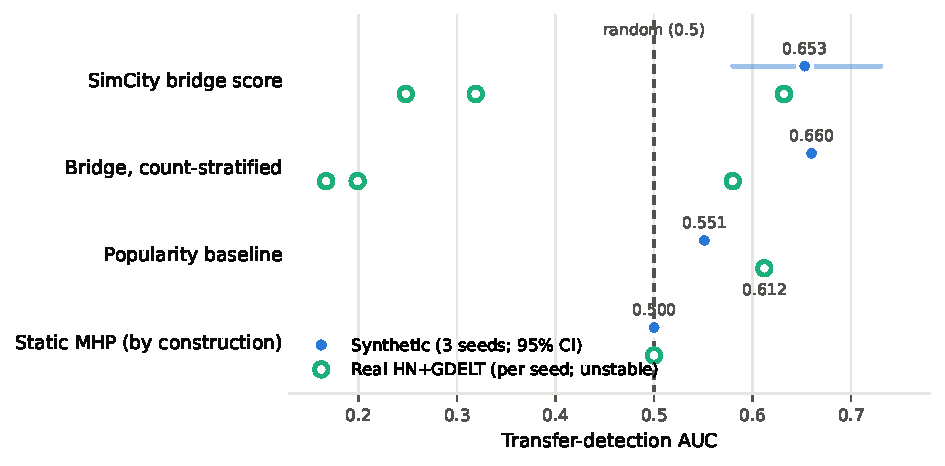
\includegraphics[width=0.92\linewidth]{figures/transfer_auc.pdf}
\caption{\textbf{Narrative transfer detection AUC}, synthetic benchmark (blue,
three seeds, bootstrap 95\% CI) vs.\ live HN+GDELT corpus (green, 95\% CI),
against the popularity baseline and the static MHP, which is random at this
task by construction. The neural bridge score is significantly above random in
both regimes and above the popularity baseline; count-stratified values control
the popularity confound.}
\label{fig:transfer}
\end{figure}

\begin{table}[t]
\centering
\small
\caption{\textbf{Narrative transfer detection} (synthetic benchmark): ranking
which single-platform narratives will later cross platforms, scored causally
from pre-switch events. AUC over three seeds; a static MHP is random by
construction. The learned score survives both the popularity and latent-reach
confounds.}
\label{tab:transfer}
\begin{tabular}{lc}
\toprule
\textbf{Scorer} & \textbf{AUC} \\
\midrule
SimCity bridge score (per-narrative $\sum_{i\neq j}\hat\alpha_{ij}/\hat\gamma_{ij}$)
  & $\mathbf{0.653 \pm 0.005}$ \\
\quad within event-count strata & $0.656$--$0.662$ \\
\quad within latent-reach strata & $0.656$--$0.661$ \\
Popularity baseline (event count) & $0.551$ \\
Static MHP (single global $\alpha$) & $0.500$ (by construction) \\
\bottomrule
\end{tabular}
\\[2pt]
\footnotesize Mann--Whitney $p < 1.1\times10^{-4}$ (every seed); bootstrap 95\%
CI $[0.58, 0.73]$. $n=209$ test narratives, 123 transfer.
\end{table}

\begin{table}[t]
\centering
\small
\caption{\textbf{Supporting metrics.} Next-platform timing (AUC, 3 seeds) and
log-engagement regression (test MAE). SimCity is consistently $\ge$ the static
baselines on timing but the margin is small; on magnitude no model beats the
naive mean, consistent with the oracle noise analysis.}
\label{tab:supporting}
\begin{tabular}{lcc}
\toprule
\textbf{Model} & \textbf{Timing AUC} & \textbf{Virality MAE} \\
\midrule
SimCity              & $\mathbf{0.610 \pm 0.005}$ & $0.848$ \\
Static MHP           & $0.605 \pm 0.000$          & --- \\
Vanilla TGN          & ---                        & $0.927$ \\
Static GNN + SEIR    & ---                        & $0.923$ \\
Naive mean           & $0.500$                    & $\mathbf{0.825}$ \\
\bottomrule
\end{tabular}
\end{table}

\paragraph{(1) Engagement magnitude is intrinsically noise-dominated --- a
negative result.} On log-engagement regression, no model (including ours)
beats the naive train-mean (MAE 0.825 vs.\ SimCity 0.848). We show this is a
property of the target, not the models: an \emph{oracle} ridge regressor handed
a leak-free recent-excitation feature achieves \emph{negative} within-narrative
residual skill ($-0.107$) and near-random surge-ranking AUC (0.507), because
next-window branching-process counts carry Poisson-scale variance. We therefore
argue engagement-magnitude regression is an ill-posed headline metric for
cascade models, and evaluate timing and transfer instead.

\paragraph{(2) Cross-platform next-event timing.} Using the conditional
intensity $\lambda_i(t_k)$ (causal, history strictly before $t_k$) to predict
which platform fires next: over three seeds, SimCity attains AUC
$0.610 \pm 0.005$ vs.\ static MHP $0.605 \pm 0.000$ --- above the static
baseline on every seed, though the margin is not significant at $n{=}3$ seeds
(Welch $p = 0.23$). Shuffling test timestamps inflates SimCity's Hawkes NLL by
$15$--$25\times$, confirming genuine temporal-order learning.

\paragraph{(3) Narrative transfer detection --- the headline result
(\cref{fig:transfer}, \cref{tab:transfer}).} We ask:
among narratives so far observed on a \emph{single} platform, which will later
jump platforms? SimCity's per-narrative mean off-diagonal branching mass
$\sum_{i \ne j} \hat\alpha_{ij}/\hat\gamma_{ij}$ (``bridge score''), computed
causally from pre-switch events only, ranks 209 test narratives (123 transfer)
with \textbf{AUC $0.653 \pm 0.005$ over three seeds} (per-seed 0.649/0.658/0.652;
95\% bootstrap CI $[0.58, 0.73]$; Mann--Whitney $p < 1.1\times10^{-4}$ on every
seed). The score survives confound controls on all seeds: AUC 0.656--0.662
within event-count strata and 0.656--0.661 within latent-reach strata, versus
0.551 for the popularity baseline. Crucially, a
static MHP has a single global $\alpha$ and \emph{cannot rank narratives at
all} (AUC 0.5 by construction): per-narrative transfer detection is a
capability added by the neural parameterisation, not a marginal improvement.
Interestingly, the learned score does not simply read back the injected latent
$b_n$ (Spearman $-0.04$); it derives transfer propensity from observed
temporal history, and retains its discrimination when both popularity and
reach are controlled.

\paragraph{(4) Transfer detection replicates on real data.} On the balanced
live HN+GDELT corpus (12{,}574 events, 46/54 platform split, 138 cross-platform
narratives; 188 test narratives, 71 transfer), the same causal bridge score
attains \textbf{AUC 0.632} (95\% bootstrap CI $[0.53, 0.73]$, Mann--Whitney
$p = 1.2\times10^{-3}$), \emph{above} the popularity baseline (0.612) and
remaining 0.580 after count stratification --- strikingly close to the synthetic
0.653. An earlier imbalanced snapshot (93/7 HN/news) had yielded only chance
performance; the effect appears once the news platform is adequately sampled,
indicating the limitation was corpus imbalance rather than the model.

\subsection{Limitations and Negative Results}
\label{sec:limitations}

We report three honest limitations. (i) The multi-task objective dilutes the
Hawkes head: with uniform Kendall weighting the neural model \emph{underperforms}
the static MHP on timing (AUC 0.576); recovering the advantage requires
up-weighting the Hawkes task ($10\times$). (ii) The real-data transfer
result (\cref{sec:results}(4)), while significant, has a wide confidence interval
($[0.53, 0.73]$, 71 transfer cases) and only edges the popularity baseline after
stratification; tightening it requires a larger corpus, which the released
accumulating collector is designed to gather. (iii) The timing margin over static
MHP, while consistent across seeds, is small on synthetic data. (iv) Results are
on a two-platform real corpus (HN + news); the third social platform (Reddit/X)
remains future work pending API access.

\subsection{Reproducibility}
All experiments run on CPU. The repository releases the generator, collectors,
training (\texttt{train.py} with seed and task-weight environment controls),
and one-command evaluations (\texttt{multiseed\_stats.py},
\texttt{narrative\_transfer\_eval.py}, \texttt{platform\_prediction\_eval.py},
\texttt{burst\_ranking\_eval.py}, oracle checks), with all tables regenerable
from \texttt{results/}.

% =============================================================
% Bibliography
% =============================================================
\bibliographystyle{plainnat}
\begin{thebibliography}{99}

\bibitem{hawkes1971spectra}
Hawkes, A. G. (1971).
\newblock Spectra of some self-exciting and mutually exciting point processes.
\newblock \textit{Biometrika}, 58(1), 83--90.

\bibitem{du2016rmtpp}
Du, N., Dai, H., Trivedi, R., Upadhyay, U., Gomez-Rodriguez, M., \& Song, L. (2016).
\newblock Recurrent marked temporal point processes: Embedding event history to vector.
\newblock \textit{KDD}.

\bibitem{mei2017neural}
Mei, H., \& Eisner, J. (2017).
\newblock The neural Hawkes process: A neurally self-modulating multivariate point process.
\newblock \textit{NeurIPS}.

\bibitem{zuo2020transformer}
Zuo, S., Jiang, H., Li, Z., Zhao, T., \& Zha, H. (2020).
\newblock Transformer Hawkes process.
\newblock \textit{ICML}.

\bibitem{gomez2011netrate}
Gomez-Rodriguez, M., Balduzzi, D., \& Sch{\"o}lkopf, B. (2011).
\newblock Uncovering the temporal dynamics of diffusion networks.
\newblock \textit{ICML}.

\bibitem{farajtabar2017coevolve}
Farajtabar, M., Wang, Y., Gomez-Rodriguez, M., Li, S., Zha, H., \& Song, L. (2017).
\newblock COEVOLVE: A joint point process model for information diffusion and network evolution.
\newblock \textit{Journal of Machine Learning Research}, 18.

\bibitem{myers2012external}
Myers, S. A., Zhu, C., \& Leskovec, J. (2012).
\newblock Information diffusion and external influence in networks.
\newblock \textit{KDD}.

\bibitem{cheng2014cascades}
Cheng, J., Adamic, L., Dow, P. A., Kleinberg, J. M., \& Leskovec, J. (2014).
\newblock Can cascades be predicted?
\newblock \textit{WWW}.

\bibitem{zhao2015seismic}
Zhao, Q., Erdogdu, M. A., He, H. Y., Rajaraman, A., \& Leskovec, J. (2015).
\newblock SEISMIC: A self-exciting point process model for predicting tweet popularity.
\newblock \textit{KDD}.

\bibitem{rizoiu2017hip}
Rizoiu, M.-A., Xie, L., Sanner, S., Cebrian, M., Yu, H., \& Van Hentenryck, P. (2017).
\newblock Expecting to be HIP: Hawkes intensity processes for social media popularity.
\newblock \textit{WWW}.

\bibitem{kobayashi2016tideh}
Kobayashi, R., \& Lambiotte, R. (2016).
\newblock TiDeH: Time-dependent Hawkes process for predicting retweet dynamics.
\newblock \textit{ICWSM}.

\bibitem{shen2014rpp}
Shen, H., Wang, D., Song, C., \& Barab{\'a}si, A.-L. (2014).
\newblock Modeling and predicting popularity dynamics via reinforced Poisson processes.
\newblock \textit{AAAI}.

\bibitem{li2017deepcas}
Li, C., Ma, J., Guo, X., \& Mei, Q. (2017).
\newblock DeepCas: An end-to-end predictor of information cascades.
\newblock \textit{WWW}.

\bibitem{cao2017deephawkes}
Cao, Q., Shen, H., Cen, K., Ouyang, W., \& Cheng, X. (2017).
\newblock DeepHawkes: Bridging the gap between prediction and understanding of information cascades.
\newblock \textit{CIKM}.

\bibitem{weng2013virality}
Weng, L., Menczer, F., \& Ahn, Y.-Y. (2013).
\newblock Virality prediction and community structure in social networks.
\newblock \textit{Scientific Reports}, 3, 2522.

\bibitem{xu2020tgat}
Xu, D., Ruan, C., Korpeoglu, E., Kumar, S., \& Achan, K. (2020).
\newblock Inductive representation learning on temporal graphs.
\newblock \textit{ICLR}.

\bibitem{trivedi2019dyrep}
Trivedi, R., Farajtabar, M., Biswal, P., \& Zha, H. (2019).
\newblock DyRep: Learning representations over dynamic graphs.
\newblock \textit{ICLR}.

\bibitem{boguna2002correlated}
Bogu{\~n}{\'a}, M., \& Pastor-Satorras, R. (2002).
\newblock Epidemic spreading in correlated complex networks.
\newblock \textit{Physical Review E}, 66, 047104.

\bibitem{pastor2015epidemic}
Pastor-Satorras, R., Castellano, C., Van Mieghem, P., \& Vespignani, A. (2015).
\newblock Epidemic processes in complex networks.
\newblock \textit{Reviews of Modern Physics}, 87, 925.

\bibitem{zannettou2017webcentipede}
Zannettou, S., Caulfield, T., De Cristofaro, E., Kourtellis, N., Leontiadis, I.,
Sirivianos, M., Stringhini, G., \& Blackburn, J. (2017).
\newblock The web centipede: Understanding how web communities influence each
  other through the lens of mainstream and alternative news sources.
\newblock \textit{IMC}.

\bibitem{wilson2020crossplatform}
Wilson, T., \& Starbird, K. (2020).
\newblock Cross-platform disinformation campaigns: Lessons learned and next steps.
\newblock \textit{Harvard Kennedy School Misinformation Review}, 1(1).

\bibitem{horta2021migrations}
Horta Ribeiro, M., Jhaver, S., Zannettou, S., Blackburn, J., Stringhini, G.,
De Cristofaro, E., \& West, R. (2021).
\newblock Do platform migrations compromise content moderation? Evidence from
  r/The\_Donald and r/Incels.
\newblock \textit{CSCW}.

\bibitem{vosoughi2018spread}
Vosoughi, S., Roy, D., \& Aral, S. (2018).
\newblock The spread of true and false news online.
\newblock \textit{Science}, 359(6380), 1146--1151.

\bibitem{deffuant2000mixing}
Deffuant, G., Neau, D., Amblard, F., \& Weisbuch, G. (2000).
\newblock Mixing beliefs among interacting agents.
\newblock \textit{Advances in Complex Systems}, 3, 87--98.

\bibitem{hegselmann2002opinion}
Hegselmann, R., \& Krause, U. (2002).
\newblock Opinion dynamics and bounded confidence: Models, analysis and simulation.
\newblock \textit{Journal of Artificial Societies and Social Simulation}, 5(3).

\bibitem{castellano2009statistical}
Castellano, C., Fortunato, S., \& Loreto, V. (2009).
\newblock Statistical physics of social dynamics.
\newblock \textit{Reviews of Modern Physics}, 81, 591.

\bibitem{kendall2018multi}
Kendall, A., Gal, Y., \& Cipolla, R. (2018).
\newblock Multi-task learning using uncertainty to weigh losses for scene
  geometry and semantics.
\newblock \textit{CVPR}.

\bibitem{rossi2020temporal}
Rossi, E., Chamberlain, B., Frasca, F., Eynard, D., Monti, F., \& Bronstein,
  M. (2020).
\newblock Temporal graph networks for deep learning on dynamic graphs.
\newblock \textit{ICML Workshop on Graph Representation Learning}.

\bibitem{kumar2019predicting}
Kumar, S., Zhang, X., \& Leskovec, J. (2019).
\newblock Predicting dynamic embedding trajectory in temporal interaction
  networks.
\newblock \textit{KDD}.

\bibitem{rozenshtein2016temporal}
Rozenshtein, P., \& Gionis, A. (2016).
\newblock Temporal PageRank.
\newblock \textit{ECML PKDD}.

\bibitem{pastor2001epidemic}
Pastor-Satorras, R., \& Vespignani, A. (2001).
\newblock Epidemic spreading in scale-free networks.
\newblock \textit{Physical Review Letters}, 86(14), 3200.

\bibitem{bremaud1996stability}
Br{\'e}maud, P., \& Massouli{\'e}, L. (1996).
\newblock Stability of nonlinear Hawkes processes.
\newblock \textit{The Annals of Probability}, 24(3), 1563--1588.

\end{thebibliography}

\appendix

\section*{Appendix A: Notation Reference}

\begin{center}
\begin{tabular}{ll}
\toprule
\textbf{Symbol} & \textbf{Meaning} \\
\midrule
$\bn(t)$ & State vector $(n_S,n_E,n_I,n_R,n_Z,n_D)$ \\
$\br_k$ & Jump vector for transition $k$ \\
$\beta(t)$ & Macroscopic SEIR-Z exposure rate \\
$\hat{\beta}_{v,c}(t)$ & TGN node-level predicted infectivity \\
$\hat{\alpha}_{ij}(t)$ & Neural Hawkes infectivity (platform $j\to i$) \\
$\hat{\gamma}_{ij}(t)$ & Neural Hawkes decay parameter \\
$\gamma_I$ & SEIR Infected-to-Recovered decay rate \\
$\sigma$ & SEIR Exposed-to-Infected activation rate \\
$\eta$ & Deffuant opinion convergence rate \\
$\zeta(t)$ & Zombie resurgence rate (Hawkes-coupled) \\
$\delta_D$ & Archival rate ($Z\to D$) \\
$\theta$ & Algorithmic boost factor for Zombie content \\
$\epsilon_p(v)$ & Platform-specific confidence bound \\
$\rho$ & Deffuant smoothing steepness \\
$\tau$ & Platform pooling temperature \\
$P(k'|k)$ & Degree-degree conditional distribution \\
$k_v(t)$ & Effective temporal degree (\cref{eq:temporal-degree}) \\
$I(v,t)$ & Dynamic influence score \\
$\hv_{\cP_i}(t)$ & Platform-level pooled embedding \\
$\mu_i(t)$ & Hawkes exogenous background rate (GDELT) \\
$|\cP|$ & Number of platforms \\
$\cP_i$ & Set of nodes on platform $i$ \\
\bottomrule
\end{tabular}
\end{center}

\section*{Appendix B: Deffuant $\rho$ Sensitivity Analysis}

The smooth Deffuant formulation (\cref{eq:deffuant}) recovers the hard-threshold
model as $\rho \to \infty$; we conjecture steady-state opinion clusters are
invariant for $\rho > 10^2$ based on the bounded-confidence literature, but a
systematic sensitivity study over $\rho \in \{10^0, 10^1, 10^2, 10^3\}$ has not
yet been run and is left as future work. No result in
\cref{sec:results} depends on the choice of $\rho$.

\end{document}